\def\sectiontitle{AI plugins}

\section{\sectiontitle}

%%%%%%%%%%%%%%%%%%%%%%%%%%%%%%%%%%%%%%%%%%%%%%%%%%%%%%%%%%%%%%%%%%%%%%%%%%%%%%%%
\def\slidetitle{Public AI repositories}

\subsection{\slidetitle}
\begin{frame}
  \frametitle{\sectiontitle}
  \framesubtitle{\slidetitle}

  Many public AI models on lots of public AI repositories

  \begin{center}
    \begin{table}
      \begin{tabular}{|c|c|c|}
       \hline
       \rowcolor{tableFirstRowColor} AI repositories & Image classification models & Mask generation models \\ [0.5ex]
       \hline
       \cellcolor{tableFirstColColor} Hugging Face & 15,593 & 176 \\
       \hline
       \cellcolor{tableFirstColColor} BioImage.IO & 1 & 32 \\
       \hline
       \cellcolor{tableFirstColColor} Cellpose &  & 21 \\
       \hline
       \cellcolor{tableFirstColColor} SAM2 &  & 8 \\
       \hline
       \cellcolor{tableFirstColColor} PyTorch Hub &  & \\
       \hline
      \end{tabular}
      \caption{Number of models per repository}
    \end{table}
  \end{center}
\end{frame}

%%%%%%%%%%%%%%%%%%%%%%%%%%%%%%%%%%%%%%%%%%%%%%%%%%%%%%%%%%%%%%%%%%%%%%%%%%%%%%%%
\def\slidetitle{Unlock theses repositories}

\subsection{\slidetitle}
\begin{frame}
  \frametitle{\sectiontitle}
  \framesubtitle{\slidetitle}

  \begin{minipage}[h!]{0.53\textwidth}
    Goal: Access external AI models in WIPP

    Work: Plugins for public repositories

    \bigskip

    Question:

    How to assess the relevance of results?

  \end{minipage}\hfill
  \begin{minipage}[h!]{0.46\textwidth}
    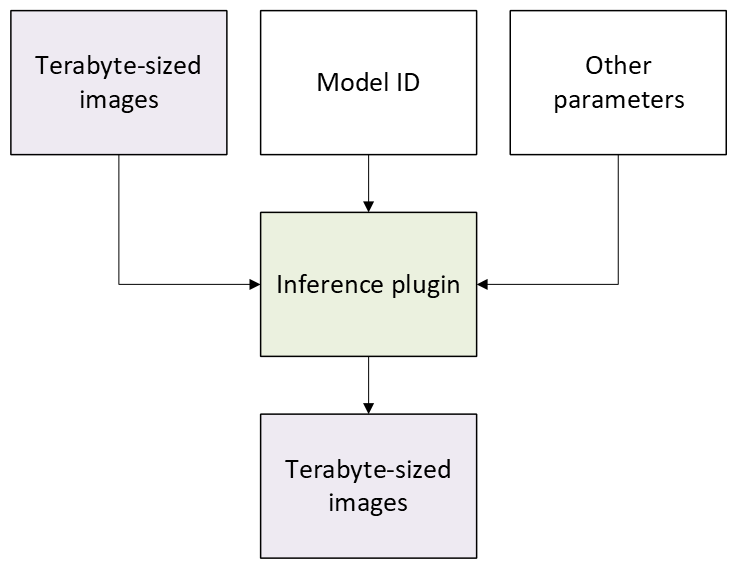
\includegraphics[scale=0.55]{./img/3_inference.png}
  \end{minipage}
\end{frame}

%%%%%%%%%%%%%%%%%%%%%%%%%%%%%%%%%%%%%%%%%%%%%%%%%%%%%%%%%%%%%%%%%%%%%%%%%%%%%%%%
\def\slidetitle{Evaluate results}

\subsection{\slidetitle}
\begin{frame}
  \frametitle{\sectiontitle}
  \framesubtitle{\slidetitle}

  \begin{minipage}[h!]{0.65\textwidth}
    Goal: Access relevance of external AI results

    \bigskip

    Work:

    Plugin to compute the Dice-Sørensen coefficient*

    \bigskip
    \bigskip

    *Statistic used to gauge the similarity of two samples
  \end{minipage}\hfill
  \begin{minipage}[h!]{0.35\textwidth}
    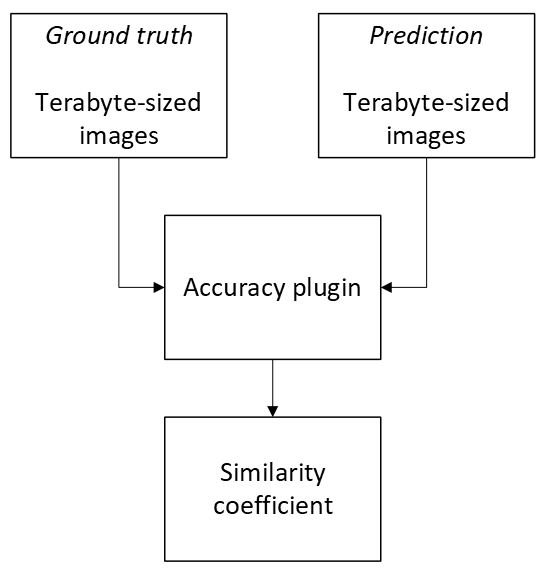
\includegraphics[scale=0.55]{./img/4_accuracy.png}
  \end{minipage}
\end{frame}

%%%%%%%%%%%%%%%%%%%%%%%%%%%%%%%%%%%%%%%%%%%%%%%%%%%%%%%%%%%%%%%%%%%%%%%%%%%%%%%%
\def\slidetitle{Benchmark example}

\subsection{\slidetitle}
\begin{frame}
  \frametitle{\sectiontitle}
  \framesubtitle{\slidetitle}

  Compute in few minutes on WIPP with dataset `3D-RPE W3`

  The first column (gray) is ground truth and the first row (blue) is model prediction

  \begin{center}
    \begin{table}
      \begin{tabular}{|c|c|c|c|c|}
       \hline
       \rowcolor{tableFirstRowColor}      & Wipp unet             & BioImage.IO*          & Cellpose cyto3        & Sam2**   \\ [0.5ex]
       \hline
       \cellcolor{tableFirstColColor} W3  & 83.97\% $\pm$ 14.95\% & 00.00\% $\pm$ 0.00\%  & 49.53\% $\pm$ 25.06\% & 30.18\% $\pm$ 27.09\% \\
       \hline
       \cellcolor{tableFirstColColor} W   & $\times$              &                       & 51.75\% $\pm$ 25.33\% & \\
       \hline
       \cellcolor{tableFirstColColor} B   & $\times$              & $\times$              &                       & \\
       \hline
       \cellcolor{tableFirstColColor} C   & $\times$              & $\times$              & $\times$              & \\
       \hline
      \end{tabular}
      \caption{Similarity across different models and ground truth}
    \end{table}
  \end{center}

  *NucleiSegmentationBoundaryModel

  **sam2-hiera-large

\end{frame}
